\chapter{Operational Information}

\section{Overview}
Classifying the picture accurately and efficiently means generating a basis upon which to relate the output of the neural network with that of a human-based classification. To generate such a basis, we need to construct three major parts:

\begin{itemize}
    \item Class Mask
    \item Training Point Pool
    \item Kernel \& Hyperplane Selection
\end{itemize}

The class mask will designate to the neural network which part of the training image belongs to which class. The training point pool is used to allow certain parts of the mask to be weighted more than other parts when training the neural network for classification. The kernel and hyperplane functions are chosen to maximize the accuracy at similar point pool sizes.

\section{Class Masking}

To classify the picture as closely as possible to the desired result, it was necessary to review the details of the image for any features that could be extracted at an elementary level. The elementary level in this case is the raw image data available through individual pixel values. The support vector machine implementation in Matlab allowed for as many classification parameters to be passed for generating the classification structure as requested. 

\begin{figure}[ht]
    \centering
    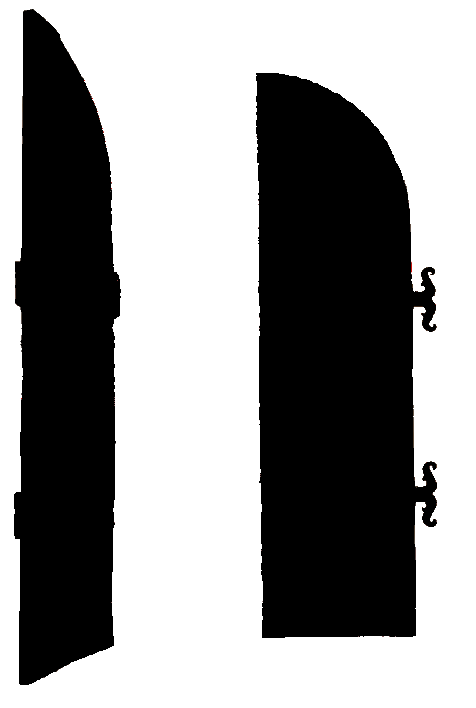
\includegraphics[height=2.5in]{00_classmask}
    \caption{Classification Mask used to determine class of training points}
    \label{fig:00_classmask}
\end{figure}

In our case, we narrowed the classification parameters down to a subset of the following:

\begin{itemize}
    \item Cartesian Coordinates (X,Y)
    \item L*a*b* pixel values
    \item Gaussian radial blur L*a*b*
    \item Sobel edge-detected L*a*b*
\end{itemize}

When using the class mask, as seen in figure \ref{fig:00_classmask}, it was necessary to generate a set of points to apply to the mask which maximized the positive effect on the support vector machine while reducing the requirement for an overly high number of required points. 

The support vector machine internally tries to maximize the distance between the points it is currently training against and the desired hyperplane\citep{SH_hyperplane0}. The pixel data at image points are known, while the hyperplane is unknown. Randomly generating points from the entire images with no concern for position doesn't benefit the areas in the image where the distinction between both classes is quite complex. This is the reason for generating points specifically in relation to the class mask. 

\section{Point Generation and Pooling}

A method for promoting certain parts of the image while also allowing for automation of point generation is shown below. By applying a Gaussian blur filter to the previous hard-edged mask, a new mask where the point densities increase relative to the distance to the mask boundary is generated. By edge-detecting and Gaussian blur filtering the class mask, the image can be extracted with ease from the class mask.

\begin{figure}[ht]
    \centering
    
\includegraphics[height=2in]{01_densitymask}
    \caption{Mask relating desired point density to position}
    \label{fig:01_densitymask}
\end{figure}

The training point generator works by sampling points through probability specified by the pixel values on this density mask. Visually the colormap, as shown in \ref{fig:02_densitymask3D}, is an example in which the points will be more likely to be generated from. For small training sizes, there is no guarantee that points will exist from those levels in the produced training set as the pool itself is sampled and culled to bring forth the final training set.

\begin{figure}[ht]
    \centering
    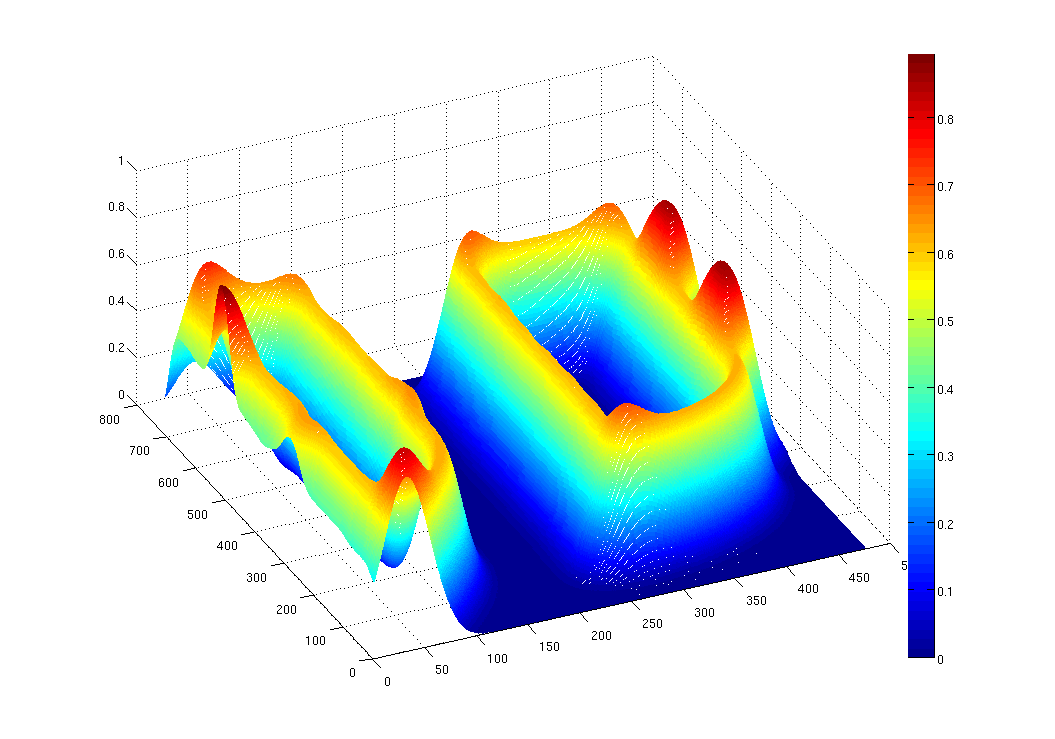
\includegraphics[height=2in]{02_densitymask3D}
    \caption{Colormap demonstrating point densities at different pixel locations}
    \label{fig:02_densitymask3D}
\end{figure}

Once we have a pool of training points with higher density point nearest the edges of the mask, we can choose a kernel function to execute the neural network with.

\section{Kernel Function}

For selecting the kernel to be used in the support vector machine, it was necessary to test those available to us from Matlab. The kernel functions available to us were as follows:

\begin{itemize}
  \item Linear
  \item Quadratic
  \item Polynomial
  \item Radial Basis Function (RBF)
  \item Multilayer Perceptron (MLP)
\end{itemize}

\begin{figure}[ht]
    \centering
    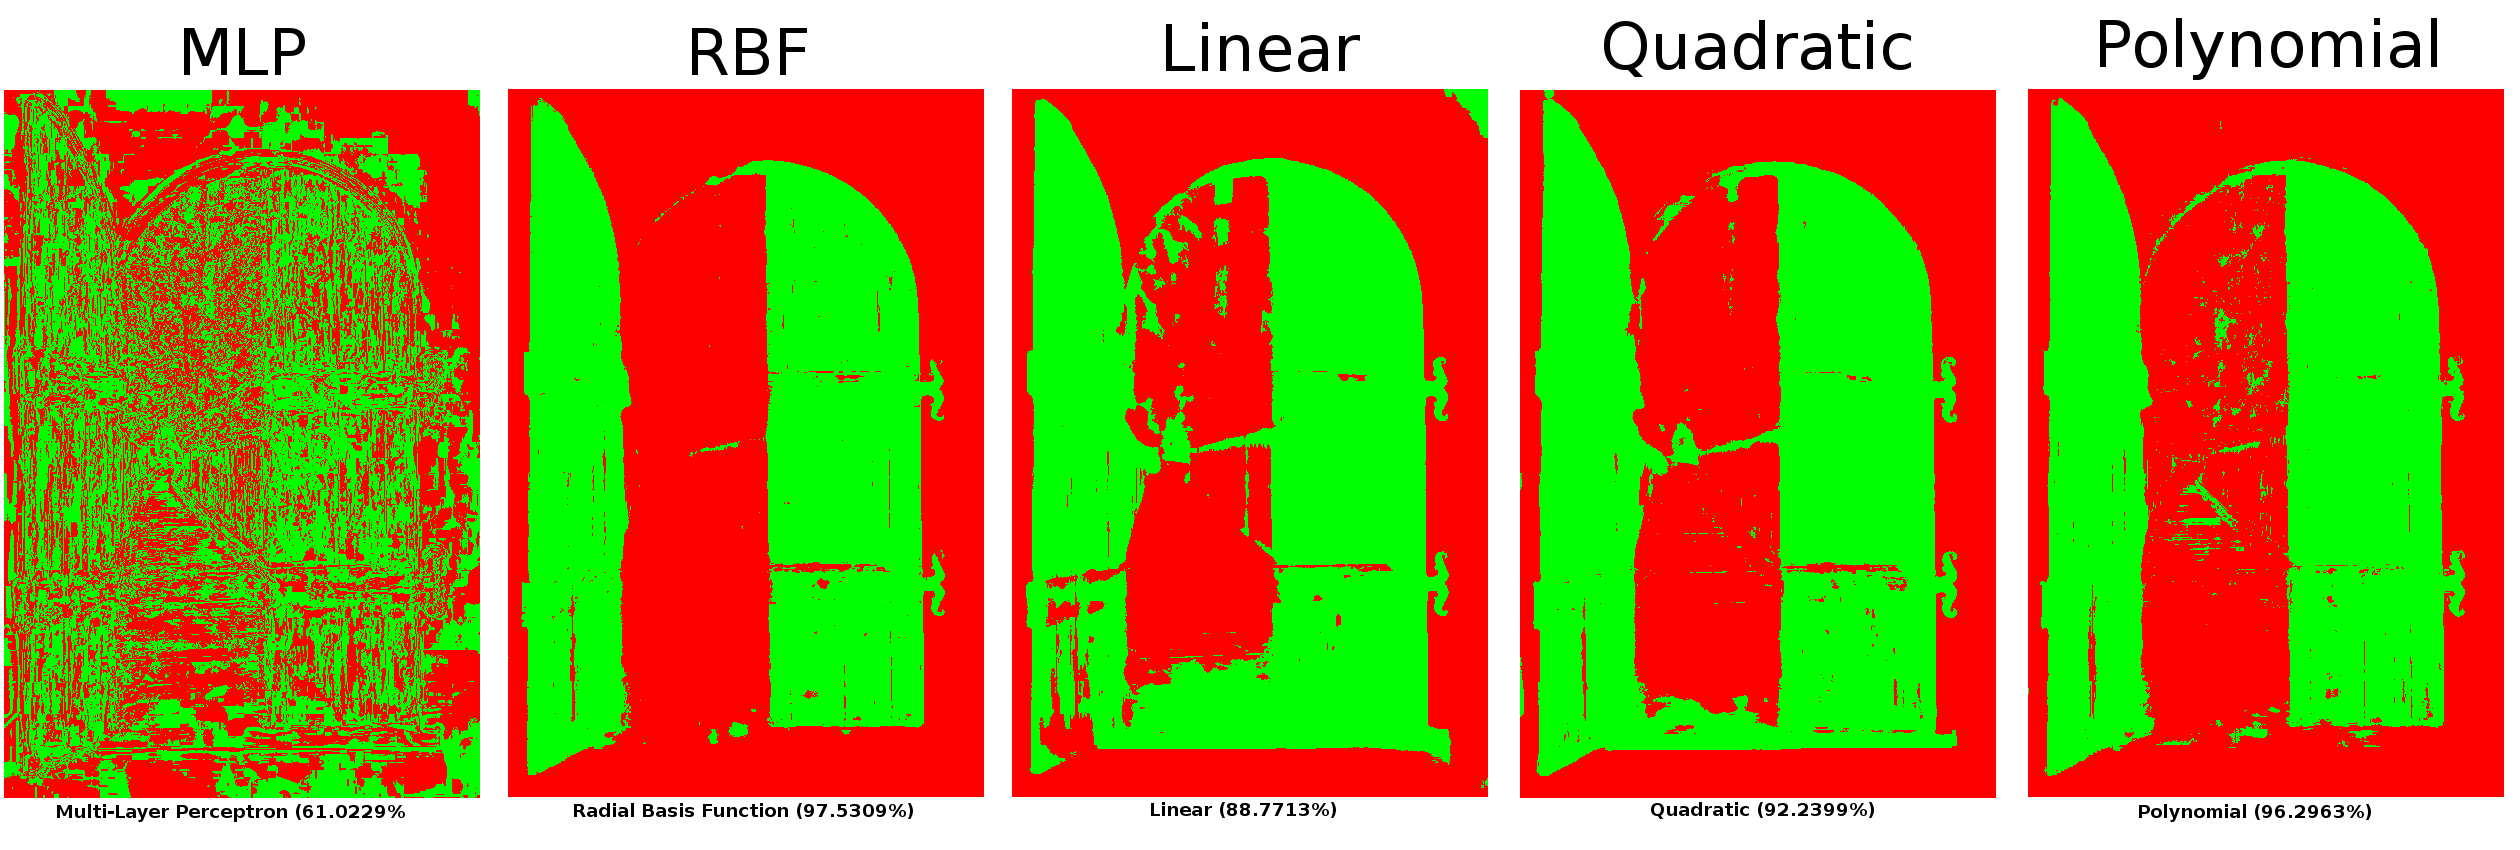
\includegraphics[width=\textwidth]{08_classifycompare}
    \caption{Comparison of the Different kernels using 1000 training points}
    \label{fig:08_classifycompare}
\end{figure}

We decided to use the RBF kernel as it worked well in conjunction with the image processing done during training. To compare the kernels, we can examine the accuracy at sampling 1000 points from the image for training. When using the MLP kernel, we noticed the accuracy dropped almost 40 percentile points for a similar calculation time to the RBF. Interestingly enough, the polynomial function was not only faster than the RBF and MLP but also had a comparable accuracy to the RBF. The quadratic kernel function had a time almost halfway between the linear and RBF kernels.

After deciding on a kernel function, it was necessary to determine a function to minimize for calculating the hyperplane.

\section{Hyperplane Method}

For the method of determining the appropriate hyperplane, we had a few choices available within Matlab. The choices available to us were:

\begin{itemize}
  \item Least Squares (LS)
  \item Quadratic Programming (QP)
  \item Sequential Minimal Optimization (SMO)
\end{itemize}

Quadratic Programming was highly resource intensive for generating a classifier in respect to both Least Squares and Sequential Minimal Optimization. When using QP, Matlab failed to finish generating the hyperplane, thus we were unable to generate a classifier with the resources we had with QP. Due to this fact, we had to exclude it from our methods.

\begin{figure}[ht]
    \centering
    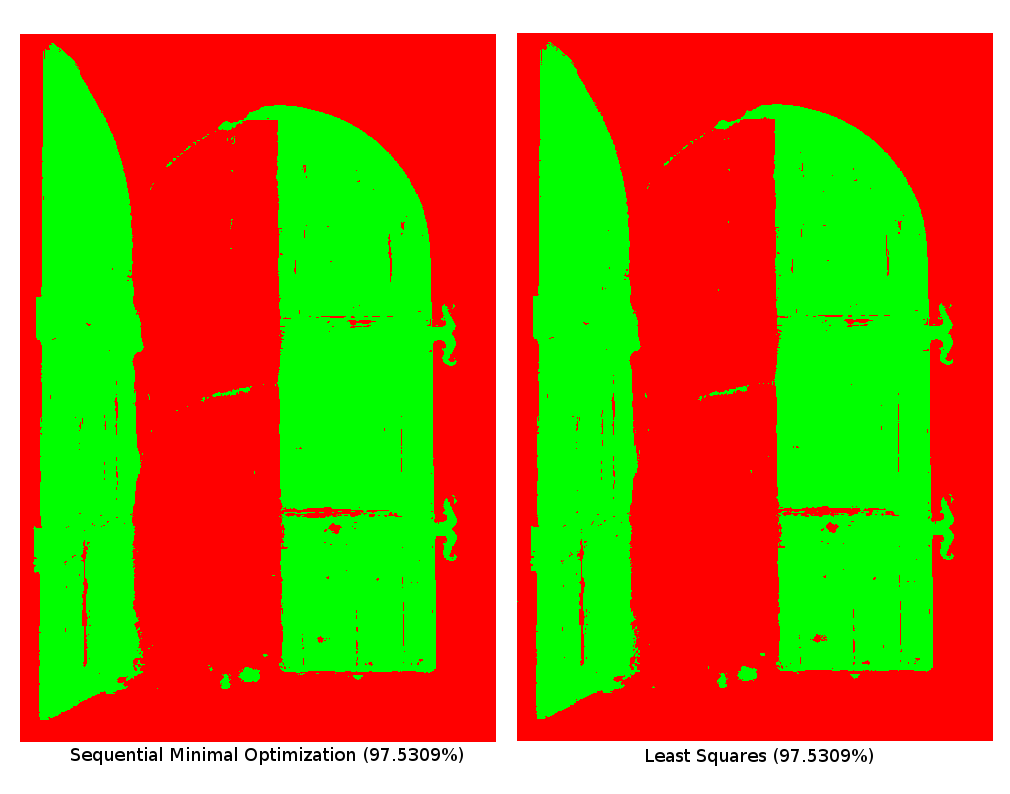
\includegraphics[width=3in]{11_lssmocompare.png}
    \caption{Comparison between methods of Least Squares and Sequential Minimal Optimization}
    \label{fig:11_lssmocompare}
\end{figure}

When comparing least squares versus sequential minimal optimization, there was no appreciable difference between the accuracies of the two. The differences between the images in Figure \ref{fig:11_lssmocompare} are very minimal, to the degree of the sixth significant digit or more. In the end, we decided to use the ``Least Squares'' method.

